% !TeX spellcheck = en_US
\chapter{State of the art}%
\gls{am} has undergone significant advancement since its inception 25 years 
ago\cite{J.Scott.2012}. Presently, \gls{am} has achieved widespread 
utilization across industries including aerospace and dentistry. 
It demonstrates versatile capabilities for processing materials 
like metals, ceramics, polymers as well as composites\cite{Frazier.2014}.
Many researchers have classified these processing techniques into the following 
categories\cite{Kruth.1991,Hartke.2011}:

\begin{itemize}
    \item \gls{vpp}
    \item \gls{mjt}
    \item \gls{bjt}
    \item \gls{mex}
    \item \gls{pbf}
    \item \gls{shl}
    \item \gls{ded}
\end{itemize}

Each process possesses its own advantages and disadvantages, 
contingent upon factors such as the materials being processed, 
construction speed, dimensional accuracy, etc\cite{Hartke.2011}.


In this work, the primary focus is the monitoring process in \gls{pbflbm}.
Hence, in this chapter, the \gls{pbflbm} technology will be
introduced, followed by an exploration of the monitoring methods employed 
in contemporary \gls{pbflbm}. Among these methods, multispectral imaging 
has been selected as the monitoring technique utilized in this work. 
Consequently, this establishes the underlying principles of the 
observation aspect within \gls{pbflbm}. Subsequently, the material's 
emissivity model will be introduced, thus leading to the current 
temperature estimation algorithms in use.
%
%
\section{Laser-based Powder Bed Fusion of Metals}
In 1989, Carl Deckard and Joe Beaman pioneered a technique 
\gls{sls}. Within this methodology, high-energy density lasers are 
focused onto the surface of metal powder, resulting in the formation of 
a solidified metal layer\cite{Mazzoli.2013,Wong.2012}. 
In the year 2002, Fisher et al. observed a phenomenon of partial melting 
in metal powders. This discovery led to the potential reduction of porosity 
in components produced through the original \gls{sls} process, subsequently 
enhancing the mechanical properties of the materials. However, it should be 
noted that complete elimination of porosity remains unattainable within the 
partial melting sintering methodolgy\cite{Fischer.2002}.


With the development of laser technology, the utilization of partial 
melting in \gls{sls} has been supplanted by the \gls{slm} approach. 
Within this technique, metal powder is subjected to complete melting, 
resulting in an elevated density of the produced part. However, 
the heightened thermal gradient inherent in this method gives rise to 
internal stresses within the finalized components\cite{Hooper.2018}, necessitating
heat treatment to alleviate these effects\cite{Osakada.2006}.


\gls{pbflb} is a type of \gls{am} process that uses a 
laser beam to selectively melt and fuse metal powder layers according 
to a digital model\cite{Swift.2013}, which includes \gls{sls} and \gls{slm}.
The structure of the \gls{pbflbm} machine can be found in Fig.\ref{fig: pbflbm}.

\begin{figure}[htbp]
    \centering
    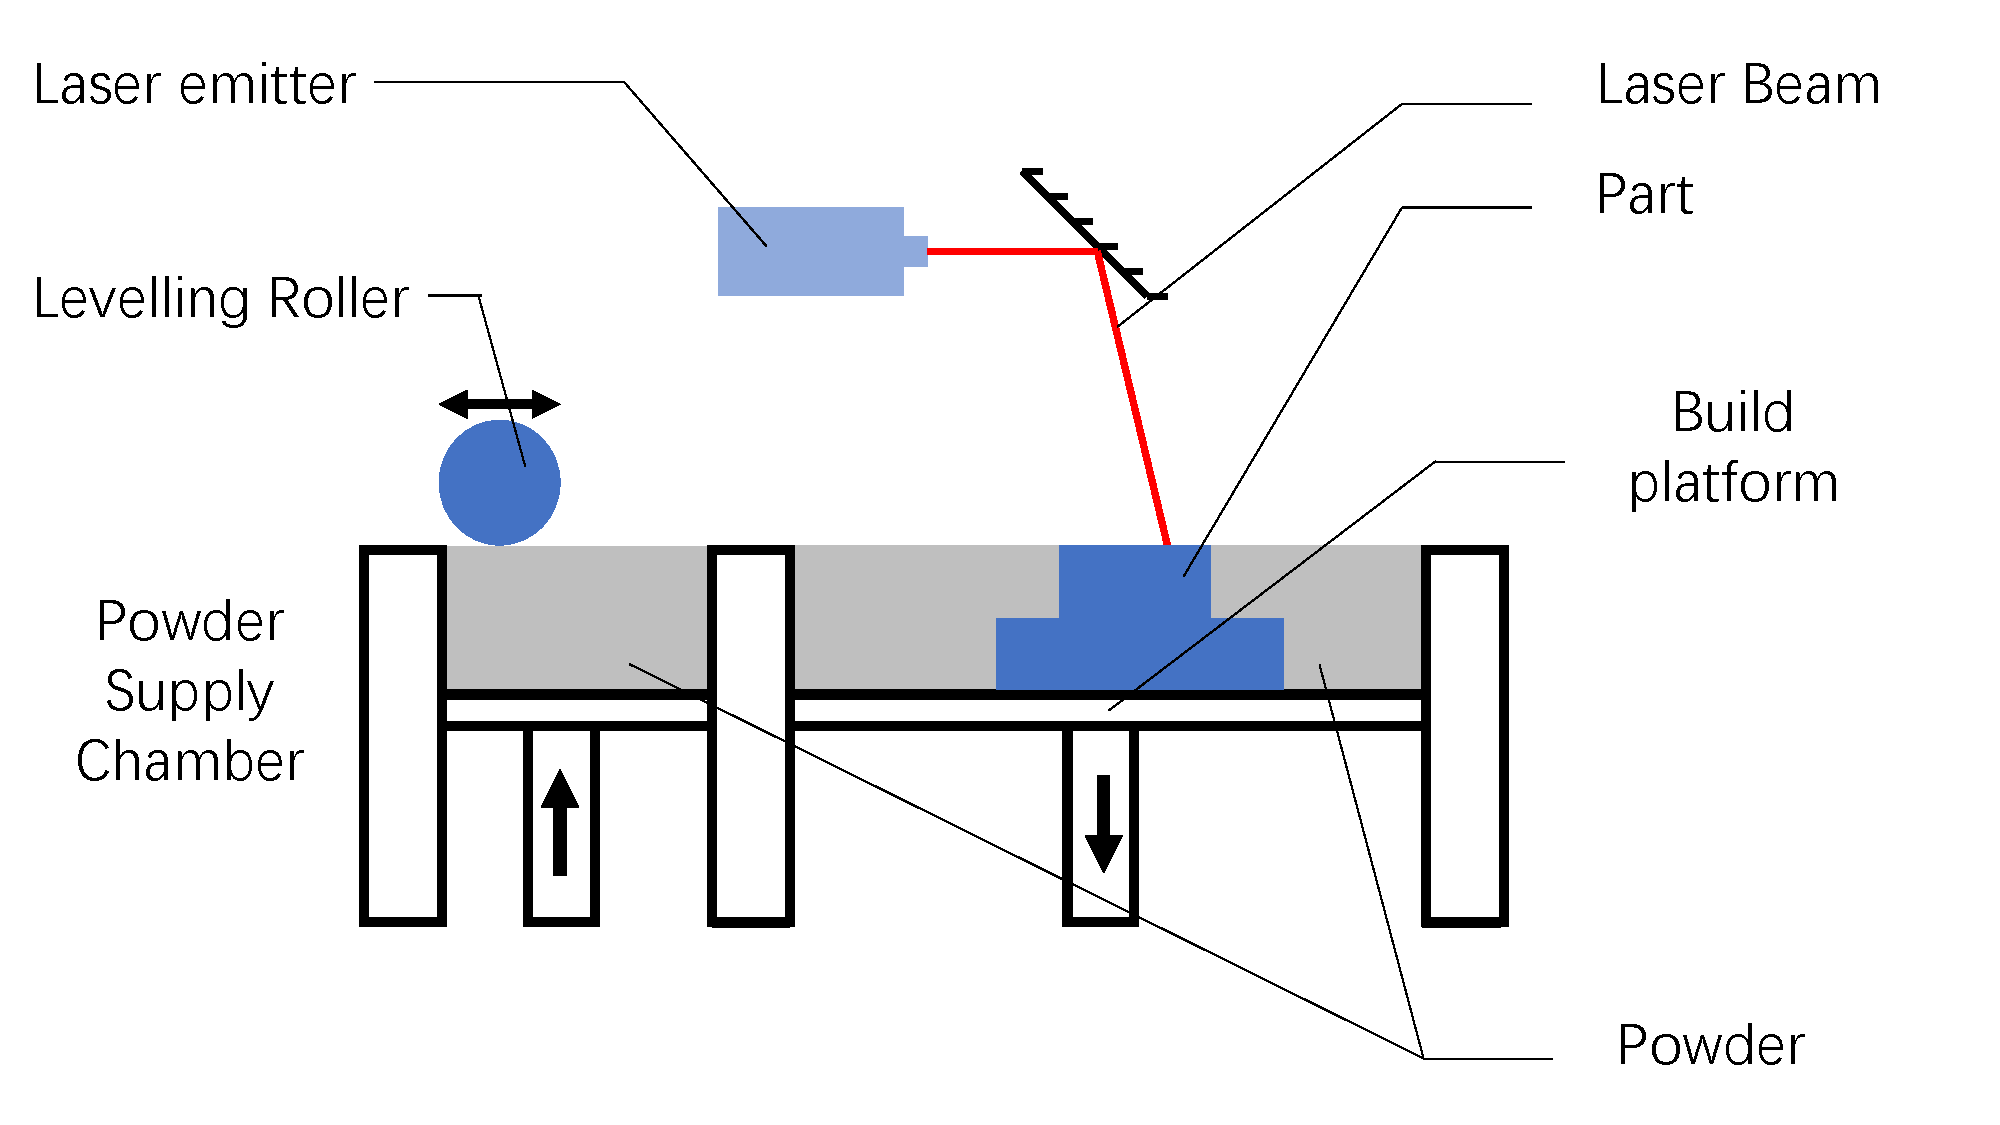
\includegraphics[width=0.9\textwidth]{figures/pbflbm.pdf}
    \caption{Laser-based Powder Bed Fusion of Metals}
    \label{fig: pbflbm}
\end{figure}


Oliverira et al. \cite{Oliveira.2020} have highlighted that two key operational parameters 
exist within the context of \gls{pbflbm}: the source power and the 
scanning velocity. These two parameters exert an influence on the energy 
density imparted to the metal powder, consequently affecting the resulting 
porosity of the fabricated product. Meanwhile, porosity stands as a 
critical parameter impacting the performance of the final product. 
The researchers \cite{Oliveira.2020} have categorized the porosity of the 
finished product into four distinct classes:

\begin{itemize}
    \item Keyhole Porosity: Excessive energy density inhibits the conduction 
    of the melt pool on the powder bed, leading the melt pool to transition 
    into a keyhole mode.
    \item Lack-of-Fusion Porosity: Insufficient energy density results in 
    incomplete fusion of the metal powder, leading to the formation of 
    porosity.
    \item "Balling" (Plateau-Rayleigh instability): Simultaneously employing 
    high source power and excessively elevated scanning velocity induces 
    instability during the processing operation.
    \item Fully-dense porosity: The ideal energy density enables the 
    component to attain a fully dense part.
\end{itemize}


Matthews et al. \cite{Matthews.2017} pointed out that in order to determine 
the evolution of the material's microstructure, information such as 
cooling rate, thermal histories, and material properties are imperative. 
This underscores the necessity of monitoring the \gls{pbflbm} process.

\section{Process monitoring}%
Li et al. \cite{Li.2019} emphasized that in-situ temperature measurement is 
of significant importance for characterizing the mechanical properties of 
materials. In-situ temperature measurement can be categorized into 
in-contact technique and non-contact technique. Given that the temperature 
of the material is high (exceeding 1000$^\circ$C), the region being heated by laser 
is small, and the cooling rate as well as the heating rate is high, 
contact-based measurements would encounter substantial interference, 
thereby rendering the obtained temperature information unreliable. 
Consequently, it becomes essential to employ non-contact-based 
temperature measurement methods.


In the realm of non-contact temperature measurement, 
various measurement systems encompassing ultrasonic, acoustic, and optical 
techniques are present. Within the context of \gls{pbflbm}, 
optical sensors are extensively utilized\cite{Krauss.2012}.


Mani et al. \cite{Mani.2017} pointed out that thermographic imaging in the 
context of Additive Manufacturing (\gls{am}) can be classified into two 
categories based on the optical pathway of the imaging system. 
One category involves aligning the field of view of the sensor with 
the laser beam\cite{Craeghs.2010b,Craeghs.2012,Chivel.2010,Bammer.2010,Berumen.2010,Lott.2011,Yadroitsev.2014}. 

\begin{figure}[htbp]
    \centering
    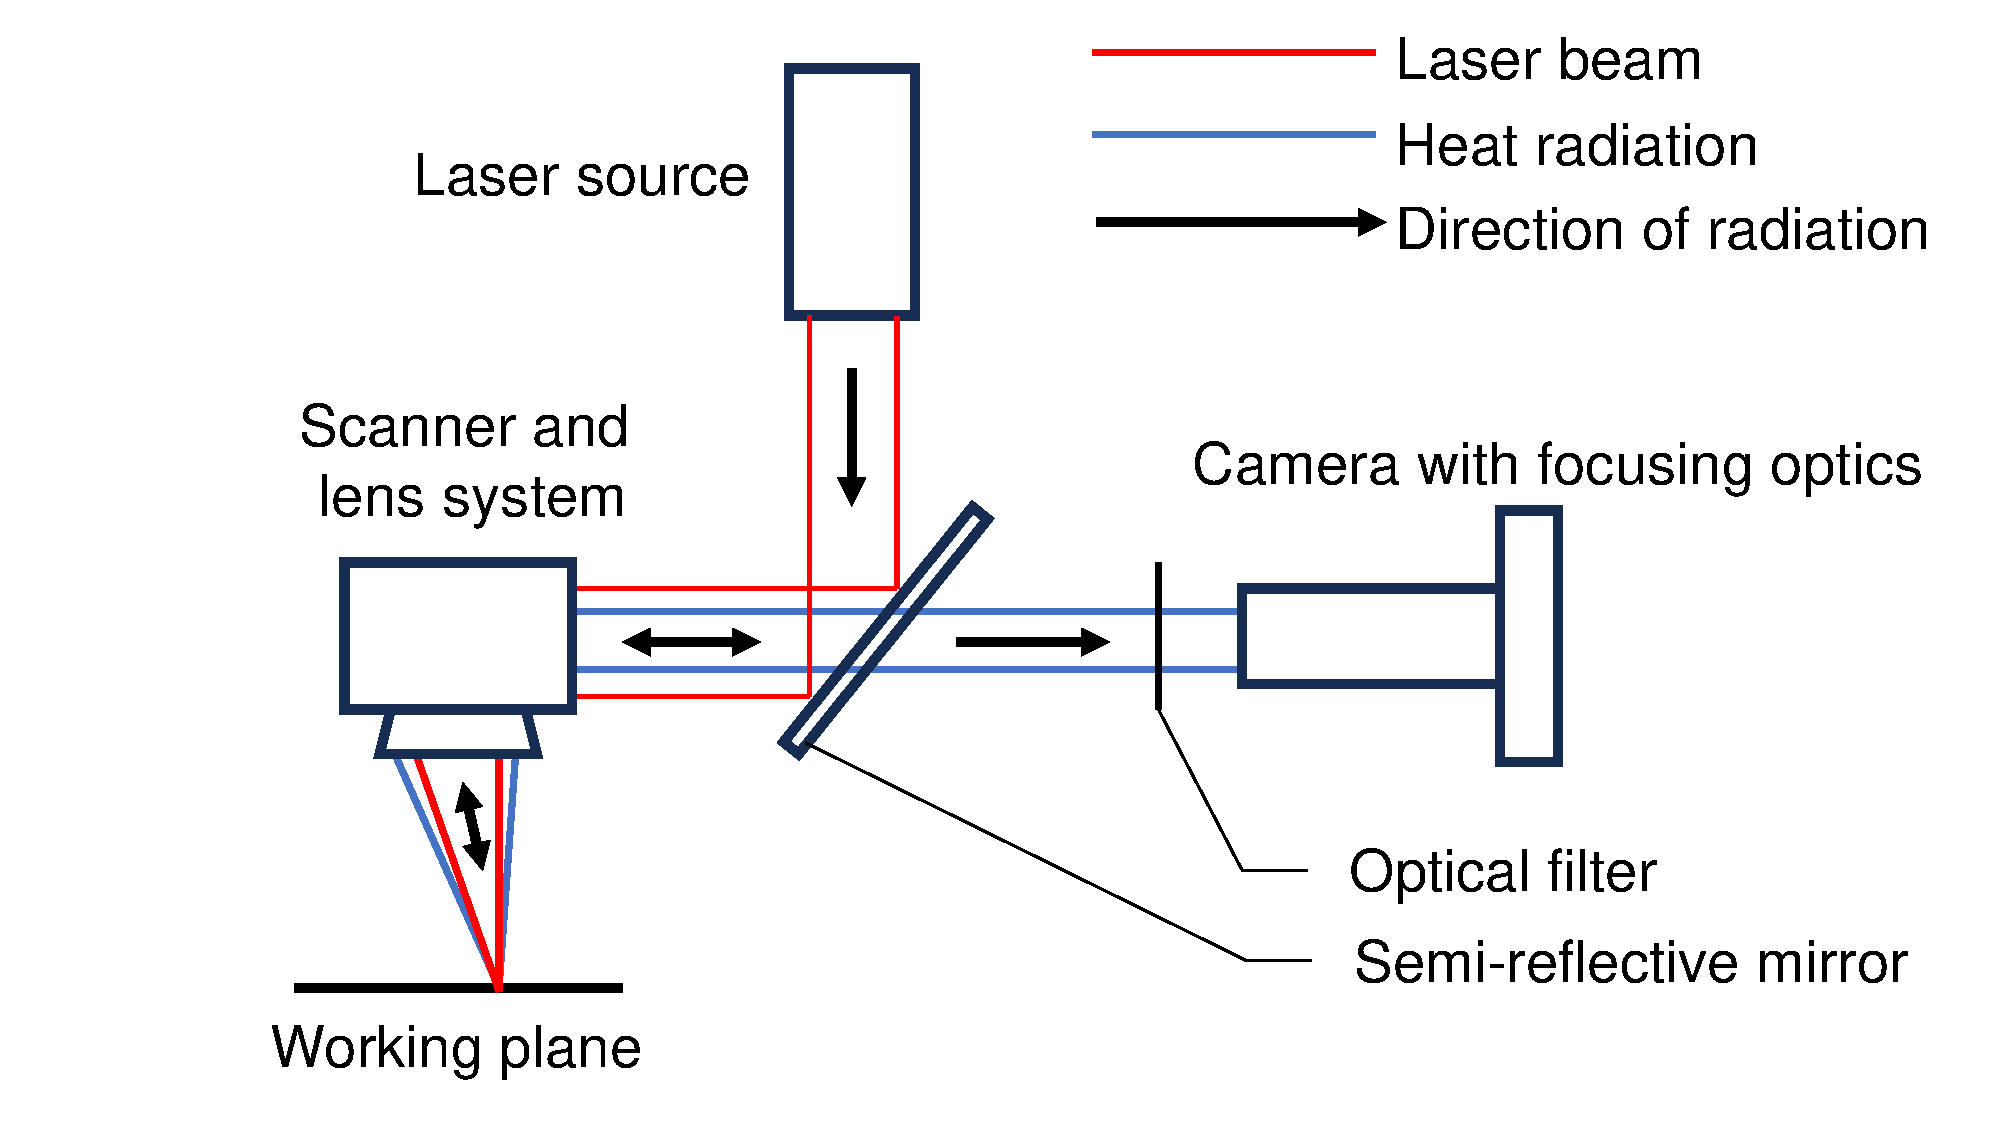
\includegraphics[width=0.8\textwidth]{figures/co-axial.pdf}
    \caption{System structure of co-axial monitoring system based on \cite{Craeghs.2010b}}
    \label{fig: co-axial}
\end{figure}

Fig.\ref{fig: co-axial} presents the structure of the measurement system. 
This alignment enables the field of view to track the laser beam, 
allowing for the observation of the melt pool and its scan trajectory.
In addition, an alternative approach involves placing the sensor 
independently of the laser beam. This configuration enables the 
field of view relative static to the material\cite{Craeghs.2012,Dinwiddie.2014,Price.2012,Price.2013,Rodriguez.2012,Wegner.2011}.
In this work, due to the use of an observation system independent of the 
laser beam in the actual experiments, the virtual experimental 
platform also features a sensor separated from the laser beam system. 
This setup facilitates system calibration and allows direct acquisition of 
sensor parameters such as quantum efficiency.


Ueda et al. designed the first infrared pyrometer (single-wavelength temperature 
measurement) to measure the temperature. This approach relies on the principles outlined in 
Planck's law, which delineates the interplay between temperature, 
wavelength, and radiative intensity, enabling the measurement of the 
temperature of the object\cite{Ueda.1986}. Subsequently, Dinwiddie et al. 
applied this method for temperature measurement in electron beam melting\cite{Dinwiddie.2014}. 
Meanwhile, Krauss et al. employed this technique to identify defects 
and discontinuous failure spots arising during the \gls{am} process\cite{Krauss.2012}.


However, due to the intricate nature of temperature in real cases, the 
single-wavelength temperature measurement approach may lead to 
misrepresentations of temperature measurement. The models employed in 
single-wavelength temperature measurement methods lack appropriate 
parameters, rendering them susceptible to interference and unable to 
accurately depict the phenomenon of changing emissivity with 
increasing wavelength\cite{Raplee.2017}.


Subsequently, the emergence of multiwavelength pyrometers became notable. 
In this technique, the intensity of radiation at two or more wavelengths 
is measured during the processing. 
Doubenskaia et al.\cite{Doubenskaia.2013}, Smurov et al.\cite{Smurov.2013b}, and Muller et al.\cite{Muller.2012} 
have achieved measurement of the melt pool using this approach. 
However, in their methods, knowledge of emissivity variation with 
wavelength is required, which is often unknown. This necessitates 
assuming a material to be a grey body, which that can lead to 
inaccuracies in temperature calculations.

Meanwhile, the multiwavelength pyrometer is limited to measuring the 
temperature at a specific point. For certain applications, 
the temperature distribution is crucial, such as detecting local hot 
spots and cold spots, as well as assessing the temperature 
distribution of the materials mentioned in this work. Consequently, the 
utilization of methods with enhanced spatial resolution becomes imperative\cite{Grujic.2023}.
To enhance the spatial resolution of temperature measurement, 
measurement systems based on cameras have been developed. 
These systems are primarily categorized into multispectral 
imaging and hyperspectral imaging. The distinction between them 
lies in the wavelength range that the sensor can capture. 
In multispectral imaging, the sensor receives discrete wavelengths, 
while in hyperspectral imaging, the sensor detects a continuous 
range of wavelengths\cite{Devesse.2017}. In this work, multispectral 
imaging was employed as the technique for temperature measurement.
%
%
\section{Multispectral imaging}%
In order to simultaneously acquire radiation information at different 
wavelengths, a beam splitting design is deemed essential. Spering et al. 
have pioneered a patented approach for achieving beam splitting 
through the utilization of a series of spectral filters\cite{Spiering.1999}. 
As shown in Fig.\ref{fig: beam_splitting}, within this system, radiation of varying wavelengths is directed towards 
different sensors. Subsequently, these sensors receive the radiation 
information, which is then amalgamated into a composite image through 
post-processing techniques. However, due to the necessity of radiation 
to traverse multiple layers of spectral filters, it becomes impractical 
to increase the number of observation channels without compromising the 
overall system performance.

\begin{figure}[htbp]
    \centering
    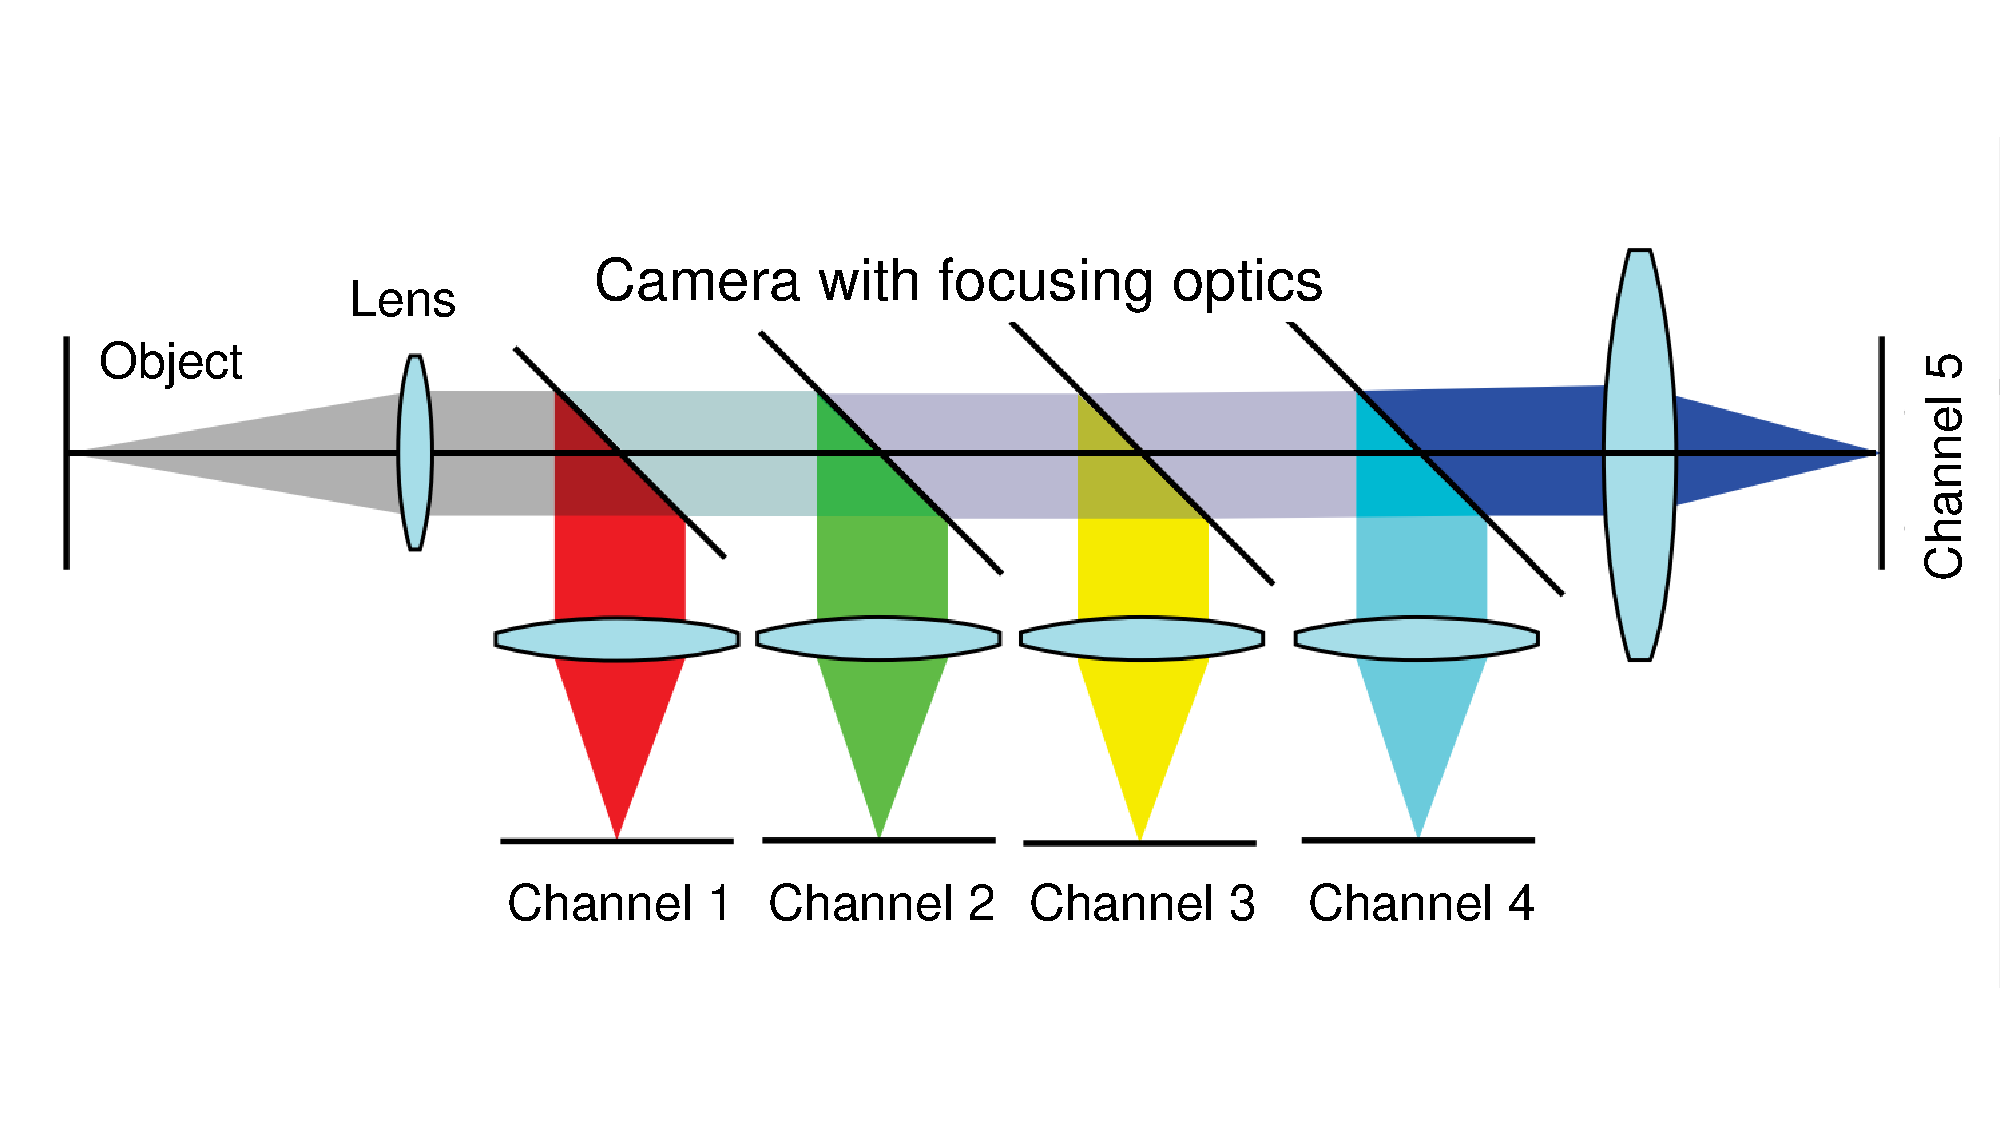
\includegraphics[width=0.95\textwidth]{figures/beam_splitting_early.pdf}
    \caption{Beam splitting structure from Spiering et al. Reproduced from \cite{Hagen.2013}}
    \label{fig: beam_splitting}
\end{figure}

With the development of camera manufacturing technology in the 1970s, 
the fabrication of single-pixel-level spectral filtering became feasible\cite{BAYERB..1976}.
Hagen et al. noted that due to the placement of all spectral filters on the 
detection layer, this design exhibits a highly compact configuration. 
However, this also introduces a drawback, necessitating the image to be 
spatially bandlimited to the Nyquist limit of the filter array. 
Failure to adhere to this requirement results in the presence of 
aliasing effects in the acquired images. Such effects can be mitigated 
by defocusing the image, thereby reducing the impact of the bandlimit 
constraint\cite{Hagen.2013}.


Due to its low utilization costs and intuitive data representation, the 
camera in the virtual experimental platform of this work employs this 
technique.

\begin{figure}[htbp]
    \centering
    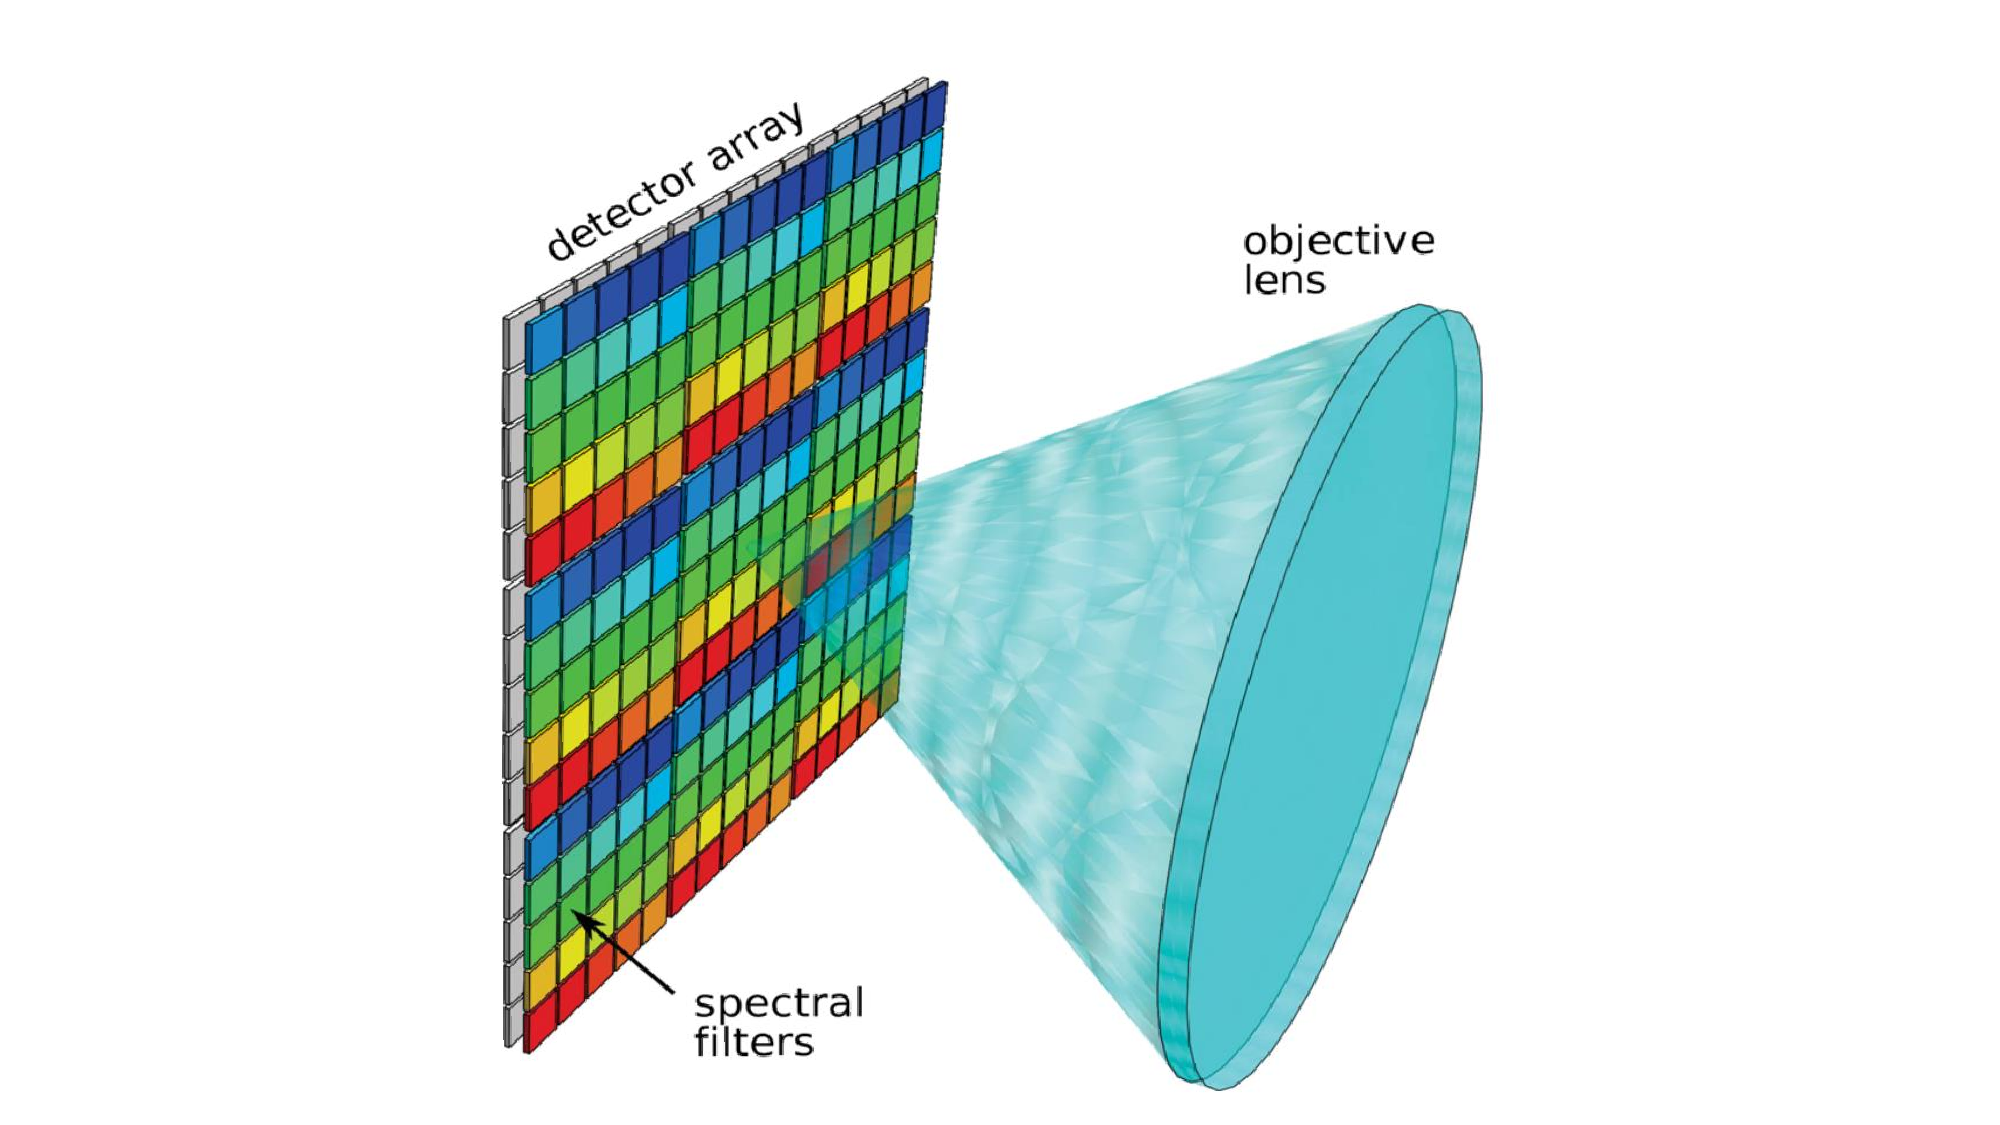
\includegraphics[width=0.5\textwidth]{figures/pixel_level_filter.pdf}
    \caption{System layout of a pixel-level filter. Reproduced from \cite{Hagen.2013}}
    \label{fig: pixel_filter}
\end{figure}

%
%
\section{Emissivity model}%

%
%
\section{Temperature estimation algorithm}


\section{Motivation of this thesis}